\chapter{Client-side user interaction}
\label{ch:client}
A client program has been realized to manipulate the dc motors directly from
the PC. It can get and set the speed of individual motors, and to apply all the
previously set speeds for all of them at once.\\ A brief list of the client's
features is given below:
\begin{itemize}
  \item Granular handling for getting and setting motors' speed
  \item Modular and extensible software architecture
  \item Terminal User Interface, implemented as a command shell
  \item Support for non-interactive use (i.e.\ scripting)
  \item Communication with master controller using the serial protocol
  \item Compatible with POSIX-compliant environments
\end{itemize}
The client is also documented with a man page, which can be found in section
\ref{sec:client-manpage}.

\section{User Interface}
The end user interacts with the whole ammc ecosystem using a text-based client.
It consists in a shell module, which I had written myself, offering some
\emph{internal commands} (hardcoded in the shell module itself) and is extended
by \emph{external commands} (found in a separated source code entity, and that
can even be compiled in a detached transaction unit).

A particular focus was made on the software architecture: indeed, every
external command can be realized standalone, and it is easy to add new
commands just by altering the \texttt{client/source/shell\_commands.c} source
file.

\section{Primitives offered}
The commands that can be used to interface with the ammc ecosystem are the
following:
\begin{description}
  \item[connect <device-path>] Connect to a master controller, given the path
    to the block device representing it.
  \item[get-speed <motor-id>] Get the speed of a dc motor given its id.
    The motor id must be specified as a decimal number.
  \item[set-speed <motor-id>=<speed>] Set the speed of a dc motor given its id.
    The motor id must be specified as a decimal number and the speed must be
    specified in rpm.
  \item[apply] Apply the previously set speed for all the dc motors.
  \item[set-slave-addr] Set a new TWI address for a slave controller.
\end{description}

\subsection{Non-interactive mode}
The client shell is capable of running in non-interactive (i.e.\ scripting)
mode with the \texttt{-s} option.  If so, it will parse the input from a
specified text file, or from \texttt{stdin} if not provided.  A shell launched
in non-interactive mode will not print shell prompts, and exit when end-of-file
is encountered or on command failure.

\section{Serial module}
The client's serial module has been realized using the POSIX \emph{termios}
interface. Unlike the master controller's counterpart, all its code is
reentrant, therefore multiple instances of multiple serial devices can
theoretically exist at the same time.

From the client's perspective, the master controller is seen as a file
descriptor, and the end user just have to specify the path of the block device
file representing the serial communication channel (e.g. \texttt{/dev/ttyACM0})
using the \texttt{connect} command.

\section{Specification}

\subsection{Software modules}
An exhaustive list of software modules for the client application is given
in table \ref{tab:client-spec-modules}. File paths are relative to the
\texttt{client/} directory.

\begin{table}[bh]
  \begin{tabularx}{\textwidth}{c X X}
    \toprule
    Module & Description & Files \\
    \midrule
    communication &
      Contains all the top-level communication routines &
      \texttt{include/communication.h},
      \texttt{source/communication.c} \\
    crc &
      Contains the CRC generation and checking routines &
      \texttt{include/crc.h},
      \texttt{source/crc.c} \\
    debug &
      Contains convenient debug facilities &
      \texttt{include/debug.h} \\
    main &
      Contains the main client application routine &
      \texttt{source/main.c} \\
    packet &
      Contains packet generation and manipulation routines &
      \texttt{include/packet.h},
      \texttt{source/packet.c} \\
    ringbuffer &
      Circular buffer implementation for the serial module &
      \texttt{include/ringbuffer.h},
      \texttt{source/ringbuffer.c} \\
    serial &
      Contains all the routines for the underlying serial communication layer &
      \texttt{include/serial.h},
      \texttt{source/serial.c} \\
    shell &
      Main program shell with built-in commands &
      \texttt{include/shell.h},
      \texttt{source/shell.c} \\
    shell\_commands &
      Contains the custom external commands to interact with the master
      controller &
      \texttt{source/shell\_commands.c} \\
    \bottomrule
  \end{tabularx}
  \caption{Client application software modules}
  \label{tab:client-spec-modules}
\end{table}

\subsection{Modules dependency graph}
The dependency graph for the client application software modules is shown in
figure \ref{img:client-deps-graph}. The \emph{debug} module is excluded. Notice
how the dependency flow goes in one direction (from top to bottom); this is the
result of the software architecture policy used.
\begin{figure}[hbp]
\begin{centering}
  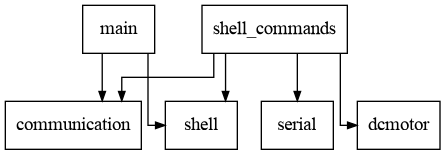
\includegraphics[scale=0.5]{client-deps}
  \caption{Client application modules dependency graph}
  \label{img:client-deps-graph}
\end{centering}
\end{figure}

\section{Man page}
\label{sec:client-manpage}
\import{./misc/}{manpage.tex}
